\documentclass[twoside]{article}
\usepackage{../../estilo-ejercicios}
\newcommand{\colapso}{{\searrow\!\!\!\!\searrow}}
%--------------------------------------------------------
\begin{document}

\title{Examen de Homología Simplicial (Junio de 2016)}
\author{Javier Aguilar Martín}
\maketitle

\begin{ejercicio}{1}
Calcular los $\F$-espacios vectoriales de homología reducida del complejo simplicial dado por la siguiente triangulación, indicando explícitamente sus generadores.
\begin{figure}[h!]
\centering
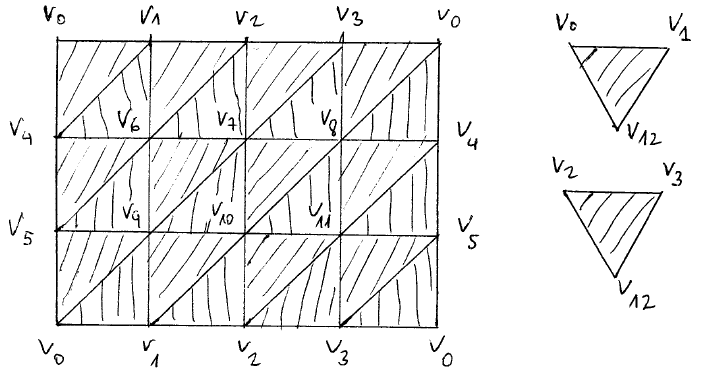
\includegraphics[scale=0.7]{Junio2016-1}
\end{figure}
\end{ejercicio}
\begin{solucion}
Denotamos $K$ a este complejo simplial. Hacemos la descomposición del complejo simplicial $K$ como $K_1=T^2$ y $K_2$ el resto. Tenemos que:
$K_2$ es colapsable, por lo que su homologías reducida también es nula.
Por otro lado:
\[ K_1 \cap K_2 = \{ v_0, v_1, v_2, v_3, (v_0, v_1), (v_2, v_3) \} \]
es decir, dos segmentos.
Luego su homología reducida es la suma de las homologías reducidas de los segmentos, que son nulas.

Esto en Mayer-Vietoris nos da que la homología reducida de $K$ es isomorfa a la del toro, y además podemos elegir los mismos generadores.
\end{solucion}

\newpage

\begin{ejercicio}{2}
Dado $n\geq p+1$, se llama $p$-collar de $k$ perlas al subespacio de $\R^n$ dado por: 
\[
C_k^p=\bigcup_{i=1}^k S_i^p
\]
donde cada $S_i^p$ es una copia de la $p$-esfera canónica. En esta unión impone que $S_i^p\cap S_j^p=\emptyset$ para todo $|j-1|>1$ y $S_i^p\cap S_j^p$ se reduce a un punto si $|j-i|=1$. Triangular un $p$-collar de $n$ perlas, calcular los $\F$-espacios vectoriales de homología reducida del citado espacio (usando la triangulación anterior), e indicar explícitamente sus generadores.
\end{ejercicio}
\begin{solucion}
Podemos triangularla como la unión de $n$ bordes de $(p+1)$-símplices uniendo dos consecutivos por un mismo vértice. Este espacio es homeomorfo a la suma punteada de $n$ $p$-esferas, por lo que sabemos que la homología de dimensión mayor o igual que 1 es la suma directa de las homologías de las esfera, teniendo en cada sumando como generador el generador de la esfera correspondiente. En dimensión 0 la homología reducida es nula por ser conexo. 
\end{solucion}


\newpage

\begin{ejercicio}{3}
Sea $K$ un complejo simplicial tal que $\dim(K)\leq 1$ y sea $v\notin K^0$. Se pide:
\begin{enumerate}[(a)]
\item Calcular los $\F$-espacios vectoriales de homología reducida de $(vK)^1$, explicitando sus generadores. 
\item Probar que $(vK)^1$ es colapsable si y solo si $\dim(K)=0$. 
\item Si $K$ es un $n$-símplice, determinar la característica de Euler de $(vK^1)^1$. 
\end{enumerate}
\end{ejercicio}
\begin{solucion}\
\begin{enumerate}[(a)]
\item Obsérvese que por construcción, $(vK)^1$ está formado por las aristas de $K$ y las aristas formadas por $v$ y un vértice de $K$. Si tenemos un 1-ciclo $(v_1,\dots, v_n)$ en $K$ (no necesariamente todos los $v_i$ distintos y se sobreentiende que después de $v_n$ viene $v_1$) entonces podemos expresar como ciclo de $(vK)^1$ de la forma $(v, v_1,v_2)+(v,v_2,v_3)+\cdots+(v,v_{n-1}, v_n)+(v,v_n,v_1)$, ya que los 1-símplices $[v,v_i]$ se cancelarán al tener orientación opuesta en cada ciclo consecutivo. Por tanto, podemos generar la homología de $(vK)^1$ con los ciclos de la forma $(v,v_i,v_j)$ donde $(v_i,v_j)\in K^1$. 
\item Si $\dim(K)=0$, entonces podemos colapsar todas las aristas de la forma $(v,v_i)$ con $v_i\in K$ sobre $v$. Si $\dim(K)>0$, entonces $K$ tiene al menos una arista $(v_i,v_j)$, luego podemos construir el ciclo $(v,v_i,v_j)$, que no es colapsable, ni puede pertenecer a un complejo colapsable porque $(vK)^1$ tiene dimensión 1. Además estos ciclos son independientes pues no es posible generar $(v, v_i,v_j)$ con otros ciclos distintos, ya que la arista $(v_i,v_j)$ solo aparece en este. De modo que $H_1((vK)^1)=\F^k$, donde $k$ es el número de aristas de $K^1$. Para $p\neq 1$, $H_p((vK)^1)=0$.
\item Por el apartado anterior, $\chi((vK^1)^1)=1-k$, donde $k$ es el número de aristas de $K^1$, que es $\binom{n+1}{2}$. 
\end{enumerate}
\end{solucion}


\end{document}
